\chapter{Background} \label{sec:background}

\glspl{ann} have shown great improvements over the last years due to increasing computational power, more sophisticated models and smarter training algorithms \cite{reboot_acgan}, \cite{unsupervised_learning_video_segmentation}. \gls{ml} and \glspl{ann} have long found their way into many commercial applications and many scientific fields have successfully applied this relatively new method of data processing to further their own research \cite{alpha_fold}, \cite{ai_medicine}, \cite{ai_antibiotic}. It was only logical that researchers and companies have also started to look into the possible benefits this emerging technology could have for Network Security applications \cite{kitsune}, \cite{ml_ids_survey}. \glspl{ann} are especially suited for \glspl{ids} due to their capability to classify data with high accuracy based on seemingly complex patterns. To harness the power of \gls{ml} for the purpose of Network Security, we made use of existing methods and models, which we will summarize in this section.

\section{Notation} \label{sec:background:terminology:notation}

Throughout the thesis, sequences are denoted $x^{(n)}$ while an element in a vector or matrix would be denoted in subscript e.g. $x_i$ or $W_{i,j}$ respectively, with matrices always written in capital letters. Superscript letters (except for $T$, which is the \textit{transpose} operator and will never be used as label) without parenthesis are part of the variable name, e.g. $W^Q$ is the \textit{query} matrix in the attention function. Deviations from this notation are stated explicitly.

\section{Machine Learning} \label{sec:background:ml}

Machine learning describes the study of computer algorithms which are \textit{trained} or \text{fitted} to optimize a given criterion without the need to specifically program them. The algorithm constructs a model based on input-output pairs which describe how the model should behave.
To ensure that the algorithm is learning patterns and structures of problems and not only memorizing input-output data pairs, the training process is often split into two phases: \textit{Training} phase and \textit{validation} phase. In the training phase, the algorithm processes the data and produces a best guess for the output. In the validation phase, the network processes unseen data, i.e. data not used during training, to ensure that the model did not just learn the training data by heart. 
Popular traditional machine learning algorithms and models used for classification are \gls{knn}, \gls{svm}, Naive Bayes or \gls{dtc}
\par

\section{Artificial Neural Networks} \label{sec:background:ann}

\glspl{ann} are a type of Machine Learning algorithm used for classification and prediction. Named after their resemblance to neurons in a brain, \glspl{ann} are systems comprised of connected nodes called \textit{artificial neurons}. Analogous to synapses, nodes communicate \textit{via} connections called \textit{edges} by sending "signals" to other nodes. Signals are represented as scalar real numbers. The output signal from a sending node is multiplied by the weight of the edge the signal is "traveling" on. Each node calculates its output signal by applying a non-linear function to the sum of its input signals. Signals travel forward through the network from the first to the last layer, but usually not within layers. The resulting computations can be summarized as a combination of function compositions and matrix multiplications $g(x) := f^L(W^Lf^{L-1}(W^{L-1}...f^1(W^1x)...))$ where $L$ is the number of layers, $W^l, l \in \{1,...,L\}$ the weights connecting nodes of the prior layer to layer $l$ and $f^l$ the activation function of the layer. $W^l$ can also be written as series $(w^l_{jk})$ where $w^l_{jk}$ is the weight between the $k$-th node in layer $l-1$ and the $j$-th node in layer $l$. \par There are various types of \glspl{ann} like \glspl{rnn} or \glspl{cnn} which have many derivations themselves but they all operate on the before stated principal of signals traveling through the network, which get transformed at each node by a differentiable non-linear function. The most popular non-linear function at this time is the \gls{relu} function. Without training, an \gls{ann} performs an input transformation that depends on the initialization values of its weights, often called \textit{parameters}. \par

%By processing the input data and comparing it with the desired output data the algorithm adjusts its internal parameters i.e. its weights through the process of \gls{sgd} to produce better results in the next iteration. 
%The influence on the output of every weight in the model is then calculated with \textit{backpropagation} \ref{sec:background:backprop} and the weights of the model are changed in the direction of the gradient. \par 

%Commonly used loss functions for regression tasks are the \gls{mae} or \gls{mse} loss or the very popular Cross-entropy loss for classification.

During training, a metric of difference, often called \textit{loss}, is then calculated between the output of the model and the ground truth, i.e. the expected output. The function used to calculate the loss is called a \textit{loss function} or \textit{cost function} and must be differentiable. The network is trained to perform a desired transformation by adjusting its weights/parameters through virtue of \textit{backpropagation} and \gls{sgd}. The network produces output $\hat{y}$ at the last layer after processing input $x$. A scalar cost/loss value is calculated by the loss function $C(\hat{y}, y)$ as a measure of difference between the networks output $\hat{y}$ and the target output $y$. For classification tasks, the loss function is usually \gls{cel}, and for regression \gls{sel} or L1 loss is typically used. Backpropagation \ref{sec:background:backprop} computes the gradient of the loss function, which is then used by a gradient method like \gls{sgd} to iteratively update all weights in order to minimize (or maximize) $C(\hat{y}, y)$. As we only aim to distinguish between attack and no-attack flows, and therefore have only two classes, we are using binary \gls{cel} with \textit{mean} reduction which is defined as:

\begin{equation}
C(\hat{y},y) = -\frac{1}{N}\sum_n^{N}[y_n \cdot log(\hat{y}_n) + (1-y_n) \cdot log(1-\hat{y}_n)]
\end{equation}

With $\hat{y}$ and $y$ being predicted, and target data and $N$ the batch size.

Other methods to train an \gls{ann} are e.g. the Conjugate gradient method or the Levenberg-Marquardt algorithm, but \gls{sgd} is by far the most popular.

\section{Stochastic Gradient Descent} \label{sec:background:sgd}

Stoachstic Gradient Descent is by far the most popular algorithm used for training modern neural networks. 
It is an iterative first-order optimization algorithm aimed to iteratively improve an objective function by updating its parameters towards its lowest point, i.e. the local maximum (or minimum). For non-stochastic gradient descent it must be possible to calculate an exact gradient. In the case of machine learning, the function to minimize is the sum (or mean) of the loss of all records in the dataset. The function, which is to be optimized, would then be $Q(\theta) = \sum^N_i C(g(x_i),y_i,\theta)$, where $N$ is the number of records in the dataset. Input $x_i$ and output data $y_i$ are seen as constants and $\theta$ represents all weights in the model. The length of the resulting gradient vector $\nabla_\theta Q(\theta)$ would therefore be the cardinality of theta $|\theta|$ which is the number of parameters used in the model. Function $f(\theta)$ is then a function that accumulates the loss for every record in the dataset. To put this into perspective: the datasets we use contain around 2 million records and the \gls{lstm} model contains 5 million weights. One can see that it is not possible for computers at this date to calculate an exact gradient. Therefore, a stochastic approach is used to estimate a gradient $\nabla_\theta \hat{Q}(\theta)$. The parameters of the objective function are then iteratively updated by a small amount towards the steepest slope, i.e. the gradient:

\begin{equation}
\theta = \theta - \eta\nabla_\theta Q(\theta)
\end{equation}

$\eta$ is called the \textit{learning rate} and is an important hyper parameter in machine learning, which must be tuned to the model and data at hand.

%If the set of all weight $\theta$ is described as $\theta = {w^l_{ij} | l \ell layers, i \ell nodes in, j \ell nodes out}$, 


\section{Backpropagation} \label{sec:background:backprop}

Backpropagation is a type of differentiation algorithm used to calculate the gradient of an arbitrary function with relatively low computational effort. 
During training, an input $x$ is processed and information is flowing \textit{forward} through the network, producing output $\hat{y} = g(x)$ \ref{sec:background:ann}, hence this is called a \textit{forward-pass} or \textit{forward-propagation}. The model output culminates into a single scalar cost after applying a loss function $C(\hat{y}, y)$, which can be interpreted as a measure of distance between the model output $\hat{y}$ and the target output $y$. For \gls{ml} the backpropagation algorithm is used to calculate the gradient of the loss function $\nabla_\theta C(\theta)$ with respect to every weight $w^l_{kj}$ in the model for the record that was processed. For this purpose, the weights $w$ are deemed parameters of the forward-propagation and inputs $x_i$ are deemed constant with the effect of $g(w)$ now only being dependent on $w$. The chain rule for differentiation is applied multiple times to calculate the partial derivative $\frac{\partial C(g(w),y)}{\partial w^l_{jk}}$ for every weight between every layer in the network, which ultimately yields the gradient of $C(g(w),y)$ with respect to $w$.

\section{Recurrent Neural Networks} \label{sec:background:rnn}

The broader concept behind all \glspl{rnn} is a cyclic connection which enables the \gls{rnn} to update its state based on past states and current input data \cite{rnn_review}. Typically, an \gls{rnn} consists of standard $tanh$ nodes with corresponding weights. There are different kinds of \glspl{rnn} like continuous-time and discrete-time or finite impulse and infinite impulse \glspl{rnn}. Here we will only look at discrete-time, finite impulse \glspl{rnn} as we will only be using those. This type of network, e.g. the Elman network \cite{rnn_elman}, is capable of processing sequences of variable length by compressing the information from the whole sequence into the \textit{hidden layer} or \textit{hidden state}. The model produces one output token for each input token, so the transformation is sequence-to-sequence where input and output sequences are of equal length. One input sequence consists of a sequence of real valued vectors $x^{(t)} = x^{(1)}, x^{(2)}, ... , x^{(T)}$ where $T$ is the sequence length. From this input sequence, an output sequence of real valued vectors $\hat{y}^{(t)} = \hat{y}^{(1)}, \hat{y}^{(2)}, ... , \hat{y}^{(T)}$ is produced. In the case of the Elman network, two parameter matrices are involved in the calculation of the output:

\begin{equation}
h^{(t)} = \sigma^h (W^h x^{(t)} + U^h h^{(t-1)} + b^h)
\end{equation}

\begin{equation}
\hat{y}^{(t)} = \sigma^{\hat{y}} (W^{\hat{y}} h^{(t)} + b^{\hat{y}})
\end{equation}

With $W^h$, $W^{\hat{y}}$ and $U^h$ being the parameter matrices, and $b^h$ and $b^{\hat{y}}$ being a parameter vectors. $\sigma^h$ and $\sigma^{\hat{y}}$ constitute (potentially different) activation functions.
To train an \gls{rnn}, pairs of input and target sequences $(x^{(t)}, y^{(t)})$ are provided, from which, analogous to the training of \glspl{ann} in general\ref{sec:background:ann}, a differentiable loss function $C(\hat{y}^{(t)}, y^{(t)})$ can be calculated which can again be minimized by applying backpropagation and \gls{sgd}. In theory, \glspl{rnn} can process data sequences of arbitrary length, but the longer the sequence, the deeper the network gets, i.e. the longer the gradient paths. This leads to complications when relevant tokens are further apart in the sequence as the \gls{rnn} is not capable of handling such "long-term dependencies" \cite{rnn_review}. Long gradient paths in \glspl{rnn} might also cause the gradient to become either very small or very large, which results in the known \textit{vanishing gradient} or \textit{exploding gradient} problems correspondingly and cause training to either stagnate or diverge. The \gls{lstm} improves upon \glspl{rnn} by making the gradient more stable and allowing long-term dependencies to be considered in the learning process.

\begin{figure}[h]
	\centering
	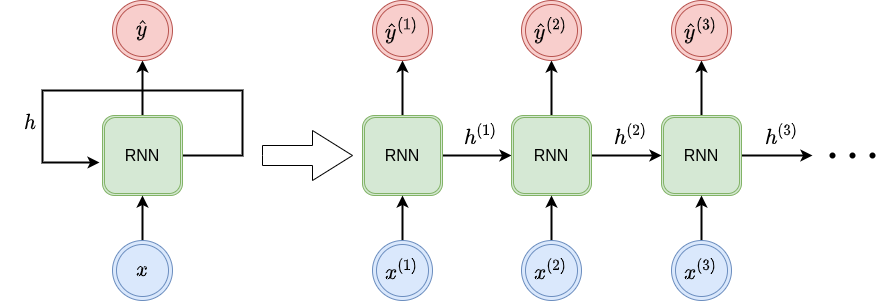
\includegraphics[width=1\textwidth]{img/recurrent_nn.png}
	\caption{Depiction of an unrolled \gls{rnn} with $x^{(t)}$ being the input sequence, $\hat{y}^{(t)}$ the output sequence, and $h^{(t)}$ the internal state of the \gls{rnn} after each processing stage.}
	\label{fig:background:rnn}
\end{figure}

\section{Long Short-Term Memory}

Introduced by Hochreiter and Schmidhuber in 1997 \cite{lstm_origin}, the \gls{lstm} model mitigates the vanishing and exploding gradient problem by replacing the $tanh$ nodes in the hidden layer of a conventional \gls{rnn} with \textit{memory cells} as seen in \ref{fig:background:lstm}. 
A memory cell is comprised of \textit{input node} $\tilde{C}$, \textit{hidden state} $h$, \textit{cell state} $C$, \textit{input gate} $i$, \textit{forget gate} $f$, and \textit{output gate} $o$. 

\begin{figure}[h]
	\centering
	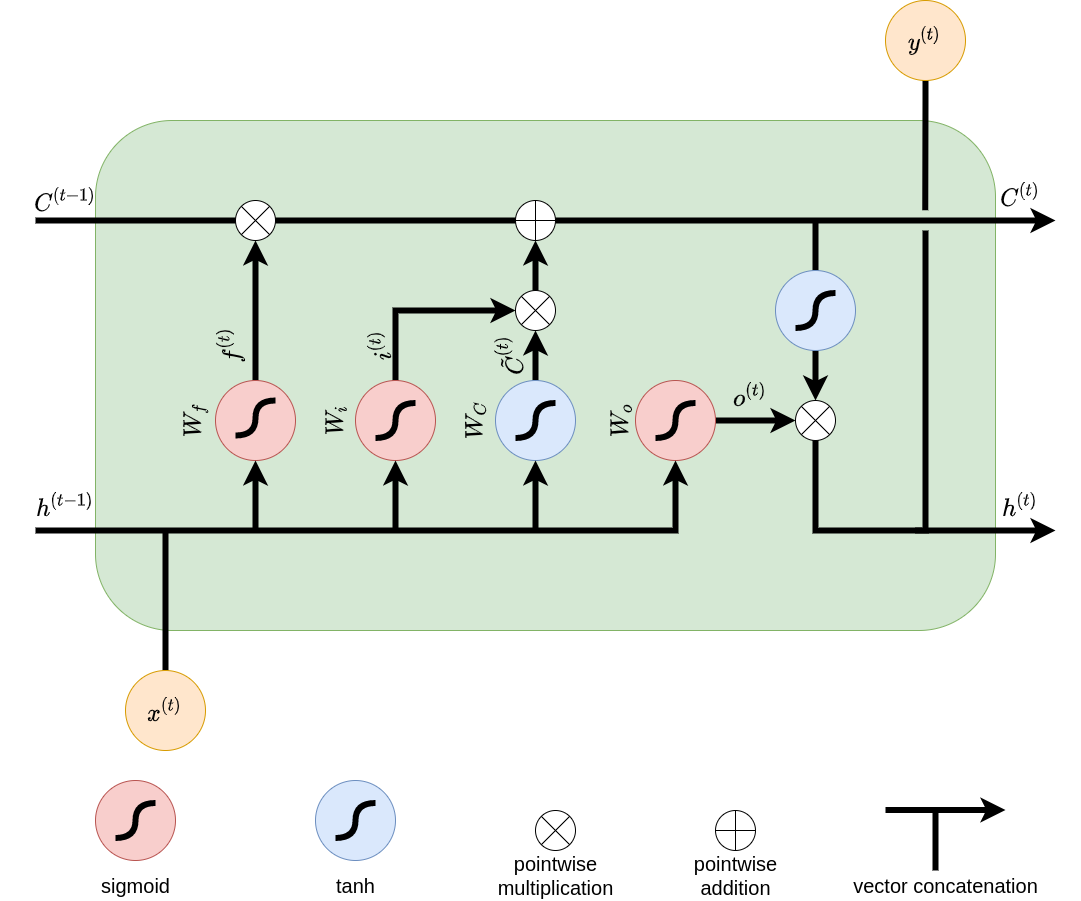
\includegraphics[width=1\textwidth]{img/lstm_cell.png}
	\caption{One \gls{lstm} memory cell \cite{rnn_zachary}}
	\label{fig:background:lstm}
\end{figure}

In contrast to an ordinary \gls{rnn}, an \gls{lstm} has two memory states: the hidden state $h^{(t)}$ and the \textit{cell state} $C^{(t)}$. Three gates enable the cell to control the flow of information and its effects on the cell state. For this purpose, gates in an \gls{lstm} consist of a point-wise multiplication with a vector that holds values between 0 and 1. The three sigma activations seen in \ref{fig:background:lstm} produce the gate vectors. The input gate $i^{(t)}$ controls whether the memory cell is updated. The forget gate $f^{(t)}$ controls how much of the old state is to be forgotten. The output gate $o^{(t)}$ controls whether the current cell state is made visible. The weight matrices $W^i, W^j$ and $W^o$ decide how information is processed by the cell and are learned parameters. The cell state is updated by addition with the vector $\bar{C}$ after multiplication with the input gate vector $i^{(t)}$. The repeated addition of a $tanh$ activation distributes gradients and vanishing/exploding gradients are mitigated.

\begin{equation}
i^{(t)} = \sigma(W^i[h^{(t-1)},x^{(t)}] + b^i)
\end{equation}

\begin{equation}
f^{(t)} = \sigma(W^f[h^{(t-1)},x^{(t)}] + b^f)
\end{equation}

\begin{equation}
o^{(t)} = \sigma(W^o[h^{(t-1)},x^{(t)}] + b^o)
\end{equation}

\begin{equation}
\bar{C}=\tanh(W^C[h^{(t-1)},x^{t}]+b^C)
\end{equation}

\section{Attention and Transformers}

In 2017, Vaswani et al. published a paper with the ominous title "Attention is All you Need" \cite{attention_origin}, referring to the already known attention mechanism which is used to model dependencies within a data sequence over longer distances. The authors proposed the transformer model consisting entirely of self attention mechanisms to model sequences and therefore diverge from the recurrent architectures of \glspl{rnn} and \glspl{lstm}. Attention is a mechanism to capture contextual relations between tokens in a sequence, e.g. words in a sentence or packets in a flow. For every token in the input sequence, an attention vector is generated, which represents how relevant other tokens in the input sequence are to the token in question. While attention can be implemented in different ways, the authors chose the scaled dot-product attention defined as 

\begin{equation}
	Attention(Q,K,V) = softmax(\frac{QK^T}{\sqrt{d_k}})V
\end{equation}

\begin{figure}[h]
	\centering
	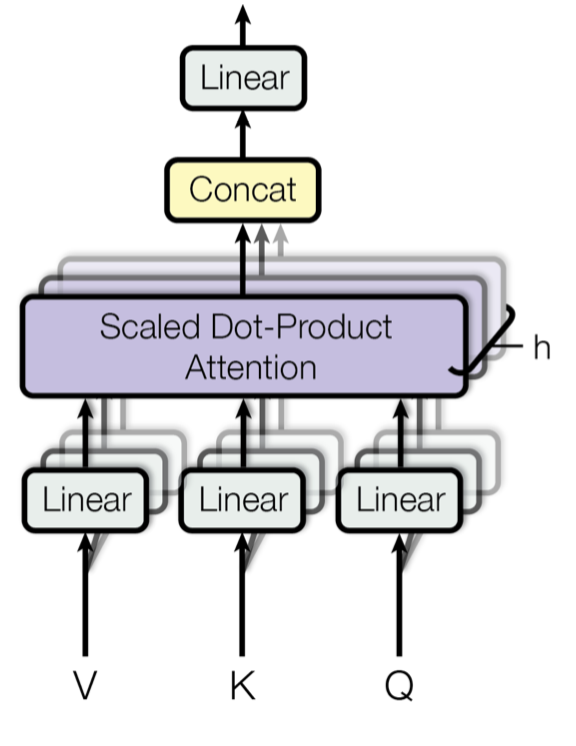
\includegraphics[width=0.3\textwidth]{img/attention.png}
	\caption{Self attention layer of Transformer by \cite{attention_origin}}
	\label{fig:attention}
\end{figure}

"An attention function can be described as mapping a query and a set of key-value pairs to an output" \cite{attention_origin}. $Q$, $K$ and $V$ are matrices composed of query, key and value vectors for every token with respect to every other token in the sequence.
Vaswani et al. proposed the use of Multi-Head Attention mechanism, suggesting the use of multiple independent attention heads which are generated by linear projection of the original $Q, K$ and $V$ matrices by different learned matrices $W^Q_i, W^K_i$ and $W^V_i$ for $i = 1, ... ,h$ where $h$ is the number of desired attention heads. The attention vectors of the different attention heads are again concatenated and projected by matrix $W^Z$ again resulting in a single combined attention vector instead of $h$ vectors. This results in the formulation 

\begin{equation}
	head_i = Attention(QW^Q_i, KW^K_i, VW^V_i), i = 1, ..., h
\end{equation}

\begin{equation}
	MultiHead(Q,K,V) = Concat(head_1, ..., head_h)W^O
\end{equation}

depicted in figure \ref{fig:attention}. The Multi-Head Attention block from \ref{fig:attention} is
used in the transformer encoder block \ref{fig:transformer_encoder} together with a fully-connected feed forward network. After each sub-layer (Multi-Head Attention, Feed Forward) layer, normalization is applied and a residual connection originating from the input to the sub-layer is added as can again be seen in figure \ref{fig:transformer_encoder}. The output of each sub-layer is hence defined as $LayerNorm(x + Sublayer(x))$ where $Sublayer$ is either a Feed Forward or a Multi-Head Attention function. While there is more to the transformer model, for our experiments we are only using the parts described here.

\begin{figure}[h]
	\centering
	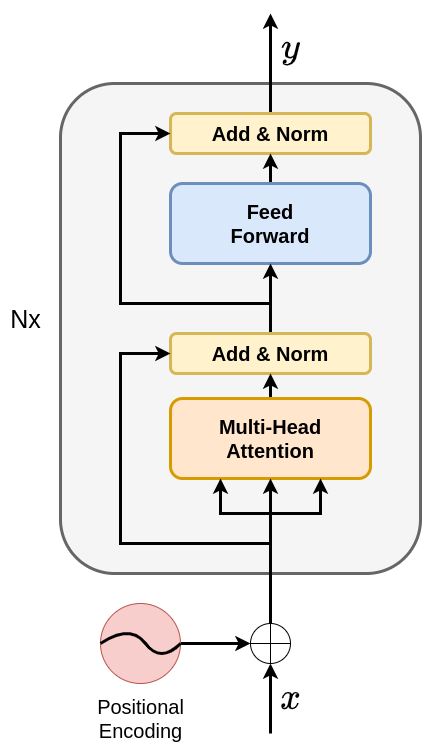
\includegraphics[width=0.4\textwidth]{img/transformer_encoder.png}
	\caption{Transformer encoder model as proposed by \cite{attention_origin}}
	\label{fig:transformer_encoder}
\end{figure}

\section{Self-supervised Learning}

Supervised learning is most effective when teaching a \gls{nn} the desired projection, but it is limited by the amount of labeled data that is available. For many use cases, not enough is available and the cost of creating new labeled data is too high to be feasible. In those cases, self-supervised learning or self-supervised pre-training might be an efficient addition or alternative. For supervised learning, the target data provides the supervision. For self-supervised learning the data itself provides the supervision, meaning the loss $C(\hat{x},x)$ is calculated between the reconstructed input $\hat{x}$ and the actual input $x$. In general this means that some part of an input tensor or an input series is withheld and the model is tasked with reconstructing the unknown information. So instead of being trained for the task, we want it to perform, it is first trained on a \textit{proxy task} which serves no purpose on its own but forces the model to learn a semantic representation, i.e. abstract features of the data which will help solve the actual task.

\section{Auto Encoder} \label{sec:backgrund:autoencoder}

The auto encoder is a popular tool for self-supervised learning. The model is composed of an \textit{encoder} and a \textit{decoder} stage as can be seen in figure \ref{fig:auto_encoder}. The encoder compresses the input data, artificially causing loss of information. In the next step the decoder tries to reconstruct the compressed data as accurately as possible. The loss $C(\hat{x},x)$ is then calculated as the difference between the original input and the reconstructed one. The aim of this seemingly nonsensical task is to force the model to form an abstract, more compact representation of the input data in its restricted latent space. To compress data with minimal loss of relevant information, the network has to find patterns in the input and ideally learns some semantic or context of the data. 

\begin{figure}[h]
	\centering
	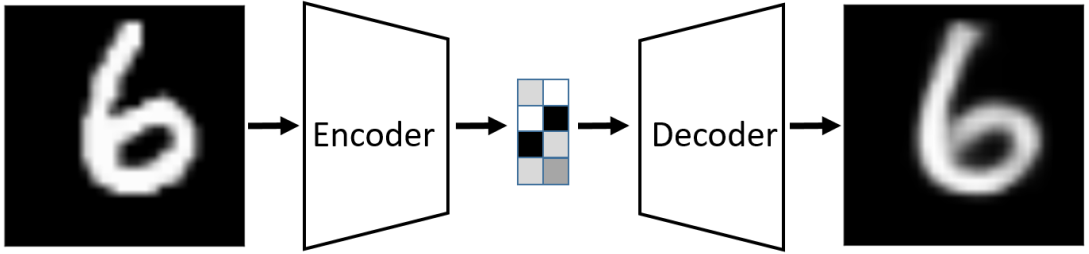
\includegraphics[width=1.0\textwidth]{img/auto_encoder.png}
	\caption{Visualization of an auto encoder. The input is encoded and subsequently decoded yielding and approximate reconstruction of the image \cite{auto_encoders}}
	\label{fig:auto_encoder}
\end{figure}

After the self-supervised training of the auto encoder is finished, the decoder stage is removed and subsequently the output of the encoder is used as input tensor for a classification or prediction model or the next layer of auto encoder. 

\section{Pre-Training and Fine-Tuning}

\textit{Pre-training} with subsequent \textit{fine-tuning} describes a methodology of training a \gls{nn} in two separate phases. E.g. Google's \gls{bert} for \gls{nlp} is pre-trained in a self-supervised fashion with vast amounts of text (3.3 billion words) \cite{bert}. \textit{Self-supervised} in this context means that the input, or parts of it, are also used as the training target. Depending on the task of the model, i.e. translation, question answering, text generation, the model's parameters are then fine-tuned with labeled data to fit the given task. \textit{Fine-tuning} then involves updating the weights of a pre-trained model by training it on a task specific labeled dataset, which is usually much smaller than the dataset used for pre-training \cite{gpt3}. Up to the release date of this paper, the pre-training - fine-tuning approach is still among the most effective approaches available when it comes to training large scale (>1 billion parameters) \gls{nlp} models, but researchers have since aimed to decrease the need for labeled data even further by only presenting the model with very few, or even just one, example of a correctly executed downstream task \cite{gpt3} instead of fine-tuning on labeled data.

\section{Performance Metrics} \label{sec:background:metrics}

To measure the effectiveness of different \glspl{ids} and machine learning models in general, a commonly used set of performance metrics has been devised to promote comparison between solutions. For binary classification (attack vs. benign), the basic metrics are

\begin{itemize}
	\item \textbf{\gls{tp}}: Number of samples correctly classified as attack
	\item \textbf{\gls{tn}}: Number of samples correctly classified as benign
	\item \textbf{\gls{fp}}: Number of samples falsely classified as attack
	\item \textbf{\gls{fn}}: Number of samples falsely classified as benign
\end{itemize}

From these basic metrics, a variety of semantically more expressive metrics can be derived, which describe different performance aspects of the classification task like overall accuracy or the rate of falsely raised alarms \cite{confusion_matrix}. Commonly used metrics are 

\begin{itemize}
	\item \textbf{Accuracy} is defined as the ration of correctly classified samples to total samples. \begin{equation}
	Accuracy = \frac{TP + TN}{TP + TN + FP + FN}
	\end{equation}
	
	\item \textbf{Precision} is defined as the ration of true positive samples to predicted positive samples and represents the confidence of attack detection.
	 \begin{equation}
	Precision = \frac{TP}{TP + FP}
	\end{equation}
	
	\item \textbf{Recall or \gls{dr}} is defined as the ration of true positive samples to total positive samples. The metric describes the probability that an attack will be detected by the \gls{ids}.
	\begin{equation}
	Recall = DR = \frac{TP}{TP + FN}
	\end{equation}
	
	\item \textbf{Specificity} is defined as the ration of true negative samples to total negative samples. The metric describes the probability that a benign flow will be categorized as such by the \gls{ids}.
	\begin{equation}
	Specificity = \frac{TN}{TN + FP}
	\end{equation}
	
	\item \textbf{\gls{fnr} or \gls{mar}} is defined as the ratio of false negative samples to total positive samples and describes how many attacks go undetected by the \gls{ids}.
	\begin{equation}
	FNR = MAR = \frac{FN}{TP + FN}
	\end{equation}
	
	\item \textbf{\gls{fpr} or \gls{far}} is defined as the ratio of false positive samples to predicted positive samples and describes how often the \gls{ids} falsely raises an alarm.
	\begin{equation}
	FPR = FAR = \frac{FP}{TP + FP}
	\end{equation}
	
	\item \textbf{F1 Measure or F Score} is calculated from the precision and recall of the test and is an alternative description of the accuracy of a statistical analysis.
	\begin{equation}
	F1 = 2*\frac{Precision * Recall}{Precision + Recall}
	\end{equation}
\end{itemize}

